% compile with: lualatex -shell-escape filename.tex
\documentclass[tikz]{standalone}
\directlua{luatexbase.add_to_callback(
  "wrapup_run",
  function() os.execute("pdf2svg \jobname.pdf \jobname.svg") print("Converted to SVG.") end,
  "final callback to convert pdf file")}

\usetikzlibrary{fit, positioning, shapes.geometric}

\pgfkeys{/pgf/.cd,
    ellipse ratio/.code={\pgfkeyssetvalue{/pgf/ellipse ratio}{#1}},
    ellipse ratio/.initial=1
}

\begin{document}

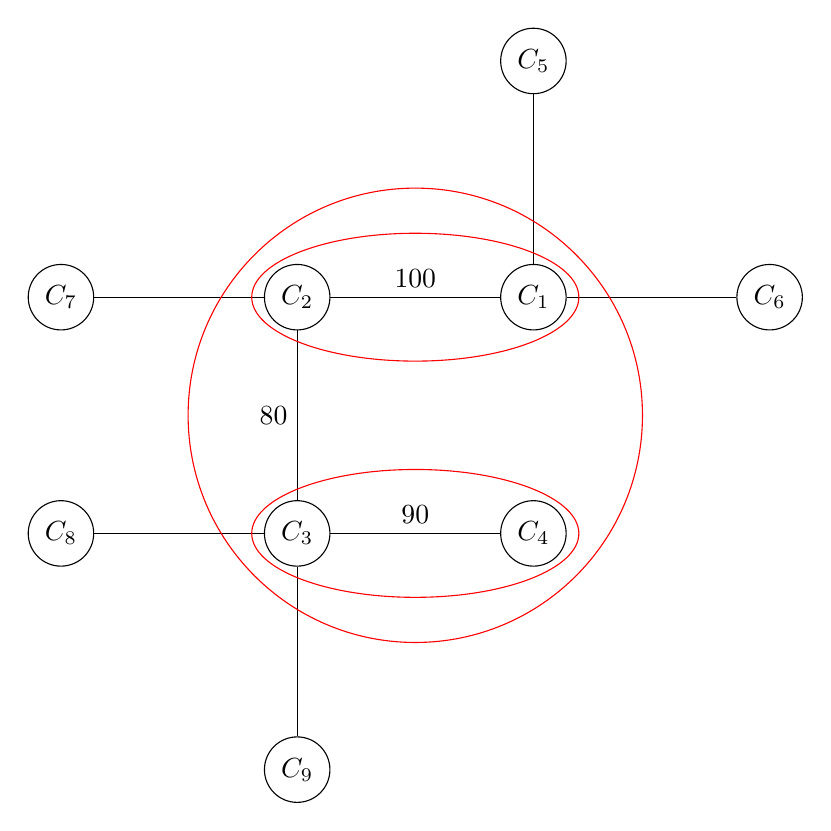
\begin{tikzpicture}[
  tree/.style={
    circle,
    draw,
  },
  level distance=30mm,
  ]

  \node[tree] (c1) {$C_1$}
    child[grow=north] {node[tree] (c5) {$C_5$}}
    child[grow=east] {node[tree] (c6) {$C_6$}}
    child[grow=west] {node[tree] (c2) {$C_2$}
      child[grow=west] {node[tree] (c7) {$C_7$}}
      child[grow=south] {node[tree] (c3) {$C_3$}
        child[grow=west] {node[tree] (c8) {$C_8$}}
        child[grow=south] {node[tree] (c9) {$C_9$}}
        child[grow=east] {
          node[tree] (c4) {$C_4$}
          edge from parent node[above] {$90$}
        }
        edge from parent node[left] {$80$}
      }
      edge from parent node[above] {$100$}
    };

    \node[fit=(c1)(c2), shape=ellipse, inner xsep=-3ex,inner ysep=1ex, draw, red] {};
    \node[fit=(c3)(c4), shape=ellipse, inner xsep=-3ex,inner ysep=1ex, draw, red] {};
    \node[fit=(c1)(c2)(c3)(c4), shape=circle, draw, red] {};
\end{tikzpicture}

\end{document}
